\subsubsection{Purpose}
Every time a payment operation has to be carried out, the system takes care to interface with the payment handler and automatically charge the user. It could happen ether when a reservation expires or when a ride ends and charges are applied.

The user will pay by the payment method specified during the registration process. If a problem during the payment operation occurs because the payment handler refuses to complete it, the user account has to be suspended and the user is notified by the system. The user is notified even if the payment operation is successful.

\subsubsection{Scenario 1}
Federico concludes his current ride and parks within the Safe Area. As soon as the system applies the current charges, the payment is performed. Since Federico has enough money on his credit card, the operation is successfully completed and a notification is sent to the user with a summary of the charges.

\subsubsection{Scenario 2}
Vladimir has just bought a new deadly-expensive smartphone with his prepaid card and rents a car in order to get home from the shopping mall. After safely parking the car and ending the ride, the system applies the current charges and tries to carry out the payment. Unfortunately Vladimir has run out of money because of the purchase of the new mobile phone. The payment handler refuses the operation and the system immediately suspends Vladimir's account and sends him a notification. As soon as Vladimir has enough money on his card, the system automatically performs the payment and unlocks his account.

\subsubsection{Use-case}
The use-case about managing payments is shown in Table \ref{manage_payments_uc}. \\
The sequence diagram describing the payment procedure is shown in Figure \ref{man_pay_sd}.

\subsubsection{Functional requirements}
\begin{enumerate}
\item The system must automatically perform payments after a ride ends and the charge is applied to the driver;
\item The system must perform payments whenever a user is fined due to a reservation expiration;
\item The system must suspend the user's account if the user cannot pay the charged amount of money;
\item The system must unlock a suspended user's account as soon as the payment can be carried out;
\item The system shall always notify the user after performing the payment;
\item The system must use the payment method specified by the user during the registration process.
\end{enumerate}

\begin{table}[H]
\begin{center}
\begin{tabular}{p{0.3\textwidth} | p{0.7\textwidth}}
\hline
Actor & Logged user, payment handler\\
\hline
Goal & Goal 6\\
\hline
Input Condition & The current charges have been applied to the user taking into account possible discounts/additional charges and fees.\\
\hline
Event Flow & 
\begin{enumerate}
\item The system interfaces to the payment handler;
\item The system waits for a positive answer;
\item As soon as the payment handler grants the money exchange, the system performs the payment;
\end{enumerate} \\
\hline
Output Condition & The system notifies the user and updates the payment history. Moreover the system unlocks the user's account if it has been previously suspended.\\
\hline
Exception & If the payment handler blocks the payment request, the system suspends the user's account, restarts from point 1 of the Event Flow and notifies the user.\\
\hline
\end{tabular}
\end{center}
\caption{Manage payments use-case}
\label{manage_payments_uc}
\end{table}

\begin{figure}[H]
\begin{center}
		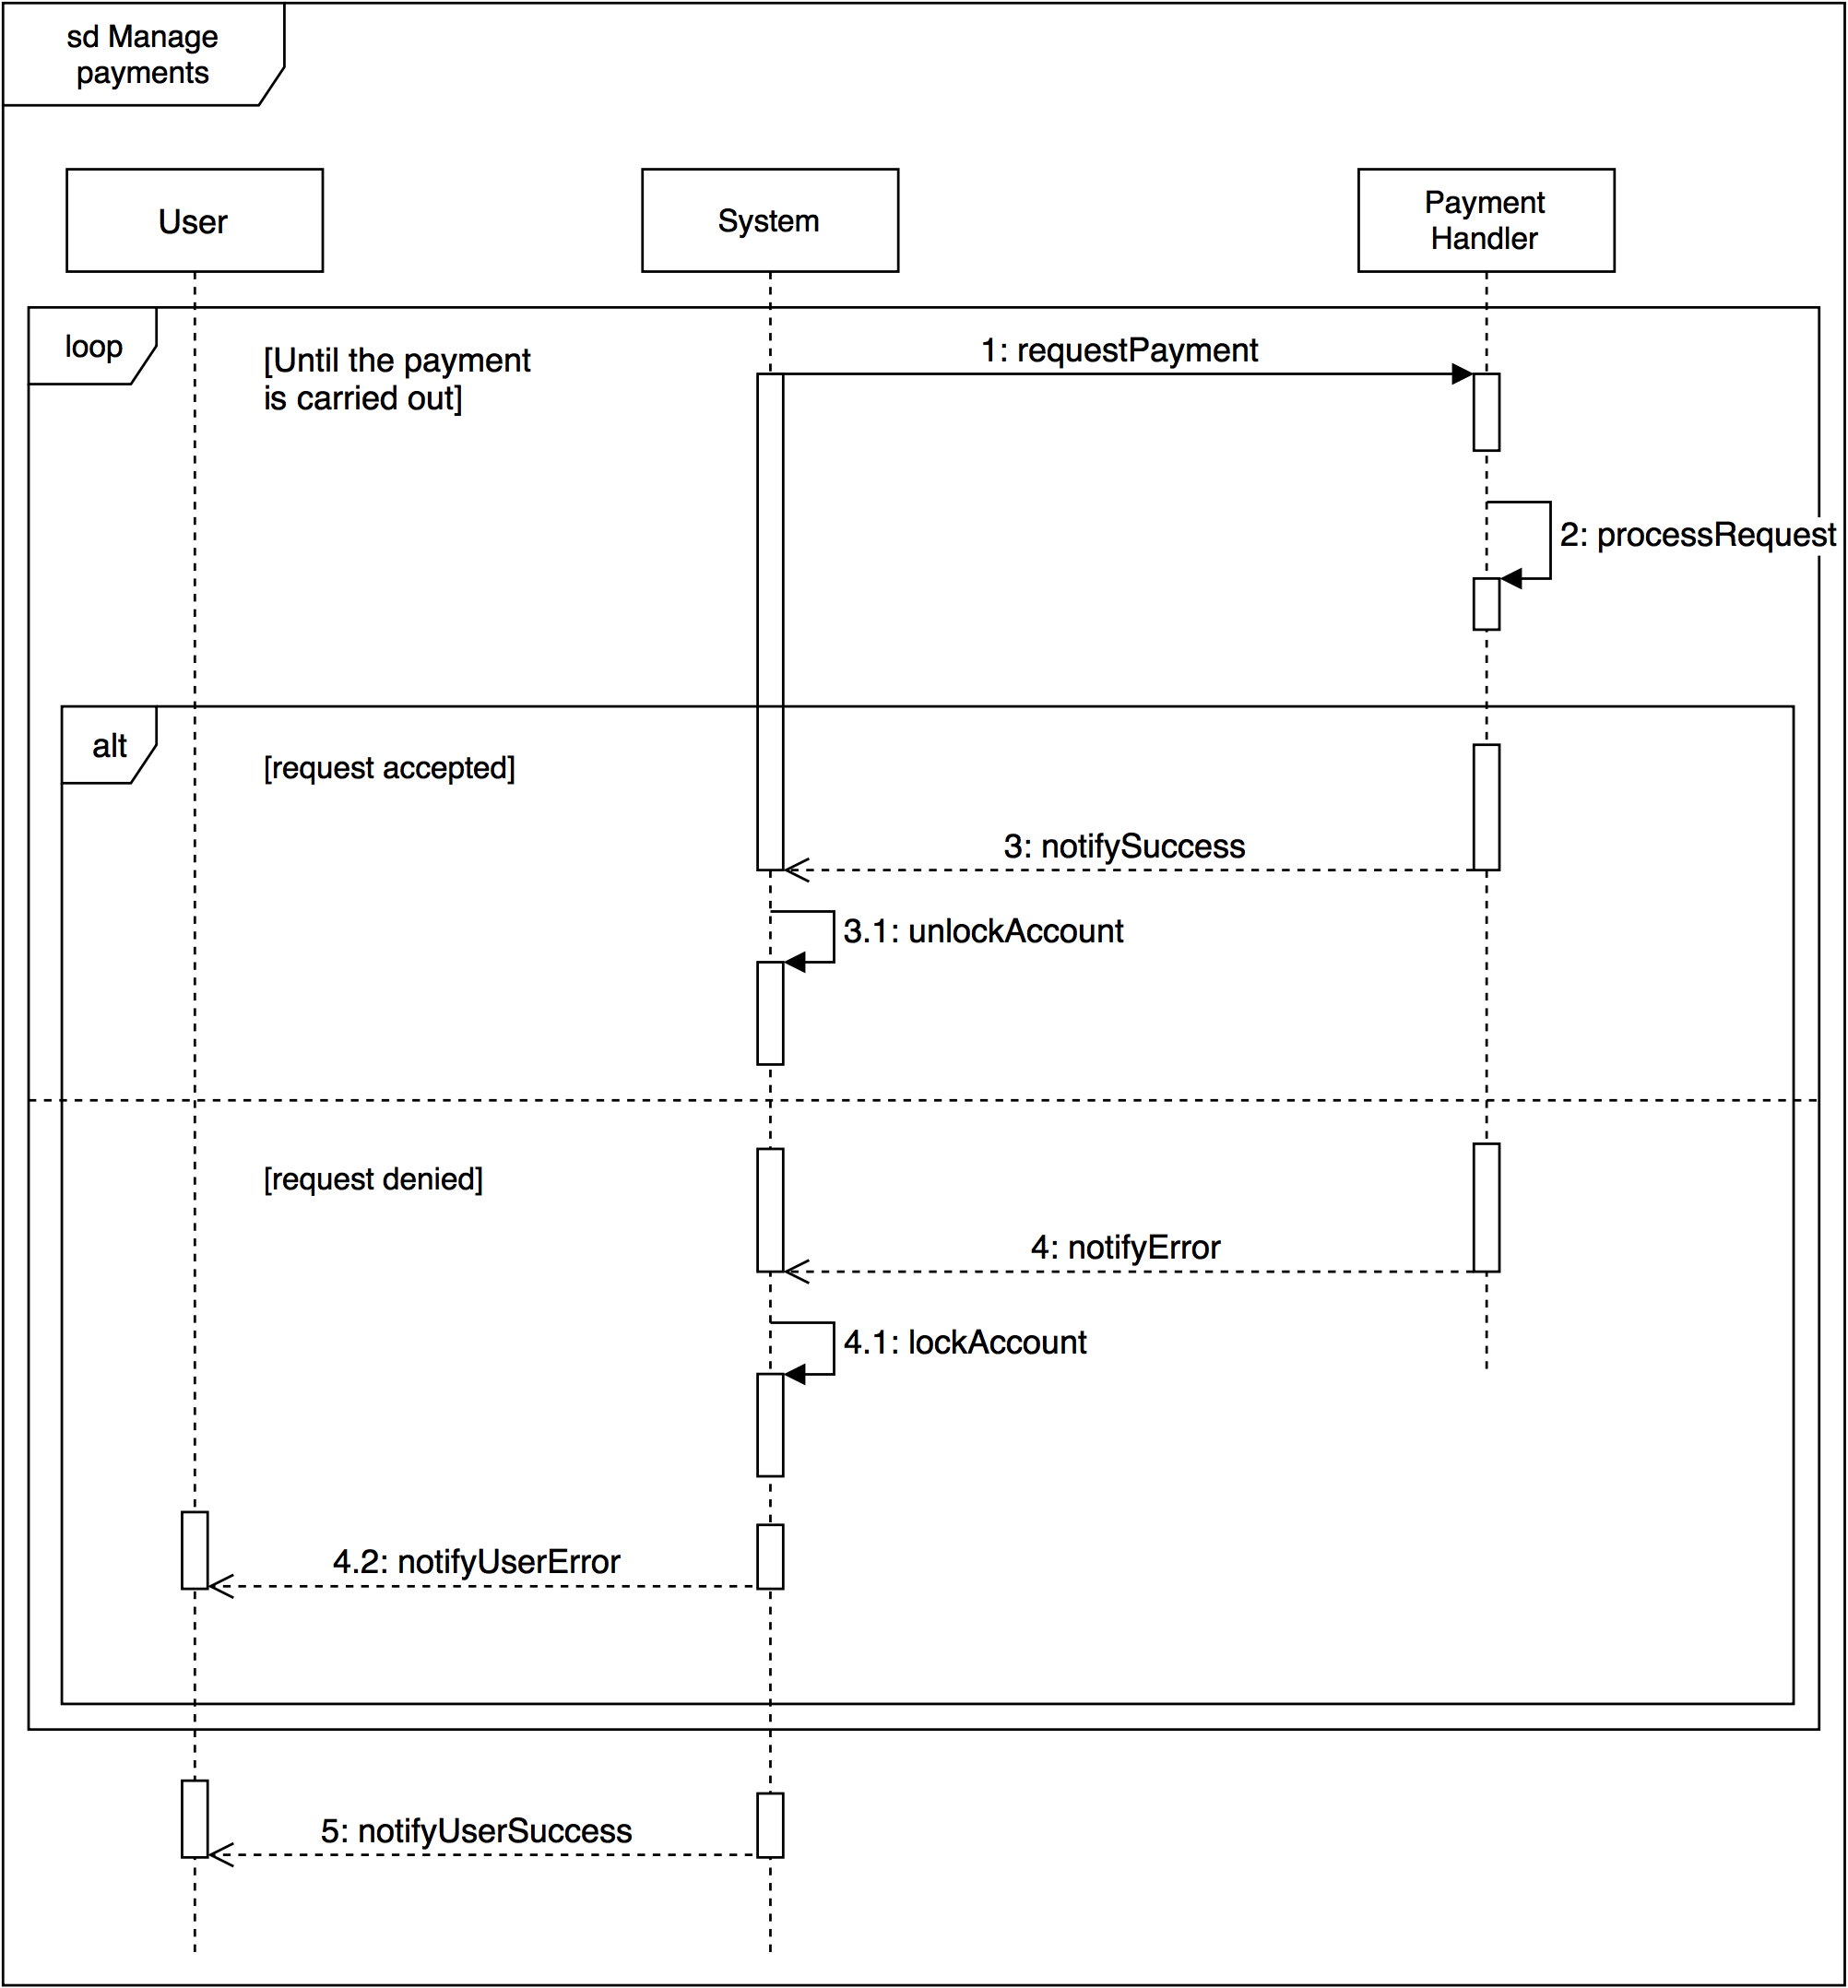
\includegraphics[width=\textwidth]{./specific_requirements/features/diagrams/manage_payments_sd.png}
		\caption{Sequence diagram of the payment procedure.}
		\label{man_pay_sd}
\end{center}
\end{figure}